
\documentclass[journal, onecolumn, 10pt]{IEEEtran}

% correct bad hyphenation here
\hyphenation{op-tical net-works semi-conduc-tor}

\usepackage{graphicx}
\usepackage{subfig}
\usepackage{amssymb}
\usepackage{amsmath} 
\usepackage[colorlinks,linkcolor=red]{hyperref}
\begin{document}

% Do not put math or special symbols in the title.
\title{Final Project of ELEC5470 FALL 2017 \\ Optimization in Image Deblurring \\ Initial Proposal}

\author{Xiaoyun~Yuan,~20322404}


% The paper headers
\markboth{ELEC5470 Final Project Xiaoyun Yuan}%
% The only time the second header will appear is for the odd numbered pages
{}
% make the title area
\maketitle

% As a general rule, do not put math, special symbols or citations
% in the abstract or keywords.
\begin{abstract}
In this report , I present some representative image deblurring algorithms and the convex/non-convex optimization techniques used in these papers. 
\end{abstract}

% Note that keywords are not normally used for peerreview papers.
\begin{IEEEkeywords}
Optimization, Image Deblurring, Prior 
\end{IEEEkeywords}

% For peerreview papers, this IEEEtran command inserts a page break and
% creates the second title. It will be ignored for other modes.
\IEEEpeerreviewmaketitle

\section{Introduction}
Nowadays, smart phone has become the digital hub of everyone's daily life, and camera is one of the most important modules on smart phones. However, limited by the space of smart phones, the smart phone camera optic system is often very simple and CMOS size is usually very small. That means the image quality is easily affected environment, for example, low light condition leads to severe noise, camera shaking and long exposure time causes uncomfortable blur effect. In this report, I focus on how to remove the image blur effects caused by camera shaking.

Image deblurring is a fundamental computer vision research problem. Now, there are two different ways to solve the image deblurring problem: 1) traditional convolutional model approach; 2) neural network approach. In this report, I mainly focus on the first approach and give some brief introductions of the second approach.

\subsection{Traditional Convolutional Model Approach}
In traditional convolutional model, the image blur effect is expressed by $2D$ convolution:
\begin{equation}
\mathbf{b} = \mathbf{l} \otimes \mathbf{k} + \mathbf{n},
\label{eqn:convolutional_blur_model}
\end{equation}
where $\mathbf{b}$, $\mathbf{l}$ and $\mathbf{k}$ are the blurry image, latent sharp/unblurred image and blur kernel respectively. $\mathbf{n}$ denotes the noise. The blur kernel $\mathbf{k}$ is usually expressed by a small matrix which is related to the camera shaking trajectory, as shown in the Fig.~\ref{fig:convolutional_blur_model}. Because the 2D convolution is difficult to handle, Eqn.~\ref{eqn:convolutional_blur_model} is often written in frequency domain:
\begin{equation}
\mathcal{F}(\mathbf{b}) = \mathcal{F}(\mathbf{l}) \cdot \mathcal{F}(\mathbf{k}) + \mathcal{F}(\mathbf{n}),
\label{eqn:convolutional_blur_model_frequency}
\end{equation}
where $\mathcal{F}(\cdot)$ denotes the Fourier transform.
\begin{figure}[h!]
\centering
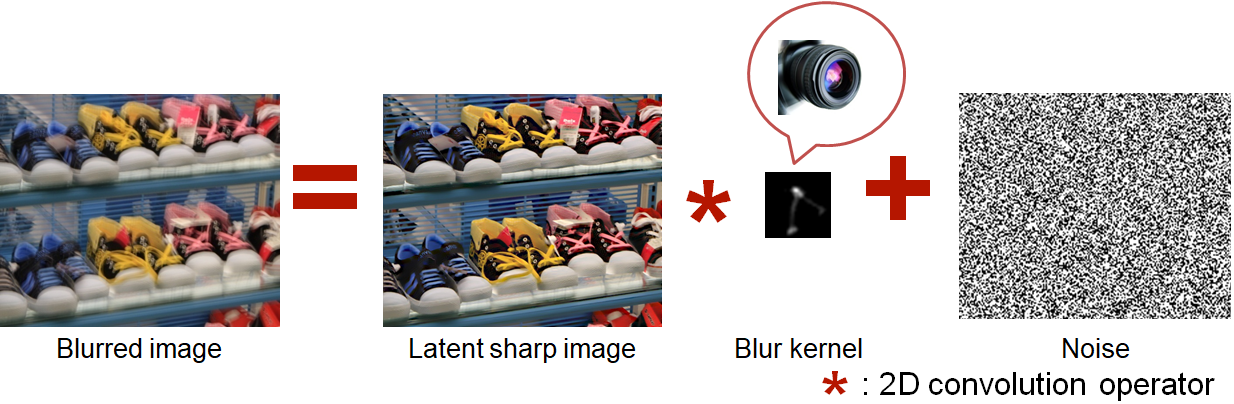
\includegraphics[width = 1\textwidth]{pic/convolutional_model.png}
\caption{Image Convolutional Blur Model}
\label{fig:convolutional_blur_model}
\end{figure}

The deblurring problem can be divide into two kinds: 1) non-blind deblurring: only $\mathbf{l}$ is unknown, use existing $\mathbf{k}$ to solve latent sharp image $\mathbf{l}$:
\begin{equation}
\min_{\mathbf{l}} \| \mathbf{b} - \mathbf{l} \otimes \mathbf{k} \|.
\label{eqn:non_blind_origin}
\end{equation}
2) Blind deblurring: both $\mathbf{l}$ and $\mathbf{k}$ are unknown:
\begin{equation}
\min_{\mathbf{l}, \mathbf{k}} \| \mathbf{b} - \mathbf{l} \otimes \mathbf{k} \|,
\label{eqn:blind_origin}
\end{equation}

The non-blind deblurring looks easy, but in fact, it is very tough in image deblurring problems. I recommend the readers to read the simple introduction \cite{deblurintro}\url{https://blogs.mathworks.com/steve/2007/08/13/image-deblurring-introduction/} first. The results are shown in Fig.~\ref*{fig:simple_inverse_filter}: (a) and (d) show the blurry image and groundtruth image respectively. (b) is the deblurring result using pseudo inverse filter. We can see that although the main structure of the image is recovered, a lot of artifacts (ringing and noise) are introduced. (c) is the result of the state-of-the-art non blind deblurring algorithm \cite{krishnan2009fast}, which I will introduce in next section.

\begin{figure}[h!]
\centering
\subfloat[blurry image and kernel]{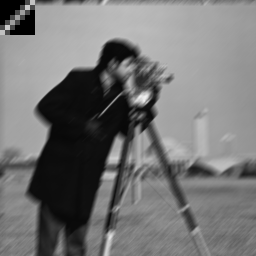
\includegraphics[width = 0.23\textwidth]{pic/cameraman_blur.png}}
\hspace{\fill}
\subfloat[pseudo inverse filter]{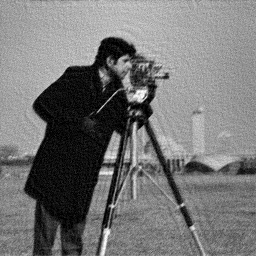
\includegraphics[width = 0.23\textwidth]{pic/cameraman_blur_pseudo_inverse.png}}
\hspace{\fill}
\subfloat[hyper laplacian $\|\nabla \mathbf{l} \|_{0.5}$\cite{krishnan2009fast}]{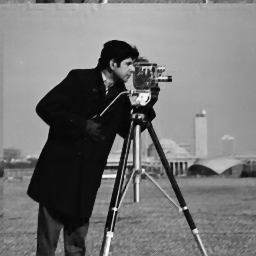
\includegraphics[width = 0.23\textwidth]{pic/cameraman_hyper_laplacian.png}}
\hspace{\fill}
\subfloat[groundtruth image]{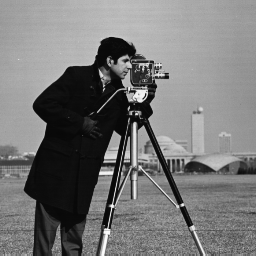
\includegraphics[width = 0.23\textwidth]{pic/cameraman.png}}
\hspace{\fill}
\caption{Image Deblurring Example}
\label{fig:simple_inverse_filter}
\end{figure}

To solve the problem is Fig.~\ref*{fig:simple_inverse_filter}(b), existing state-of-the-art algorithms usually solve the following optimization problem with image prior $\phi$ and kernel prior $\rho$ instead of original one: 1) Non-blind deblurring
\begin{equation}
\min_{\mathbf{l}} \| \mathbf{b} - \mathbf{l} \otimes \mathbf{k} \| + \lambda\phi(\mathbf{l}).
\label{eqn:non_blind_with_prior}
\end{equation}
2) Blind deblurring
\begin{equation}
\min_{\mathbf{l}, \mathbf{k}} \| \mathbf{b} - \mathbf{l} \otimes \mathbf{k} \| + \lambda\phi(\mathbf{l}) + \mu \rho(\mathbf{k}).
\label{eqn:blind_with_prior}
\end{equation}

Usually, Eqn.~\ref{eqn:blind_with_prior} will be split into two minimization problems and solve  $\mathbf{l}$ and $\mathbf{k}$ alternatively:
\begin{equation}
\begin{cases}
\min_{\mathbf{l}}&\| \mathbf{b} - \mathbf{l} \otimes \mathbf{k} \| + \lambda\phi(\mathbf{l}) \\
\min_{\mathbf{k}}&\| \mathbf{b} - \mathbf{l} \otimes \mathbf{k} \| + \mu \rho(\mathbf{k})
\end{cases}
\label{eqn:blind_with_prior_alternative}
\end{equation}


\subsection{Neural Network Approach}
The convolutional model looks very beautiful, but solving it is really not easy. Therefore, some researchers proposed to use neural network to predict the latent sharp image directly. For example, the neural network in Fig.~\ref{fig:deep_video_deblurring_cnn} takes the stacked nearby videos frames as input, and directly output the deblurred central video. 

\begin{figure}[h!]
\centering
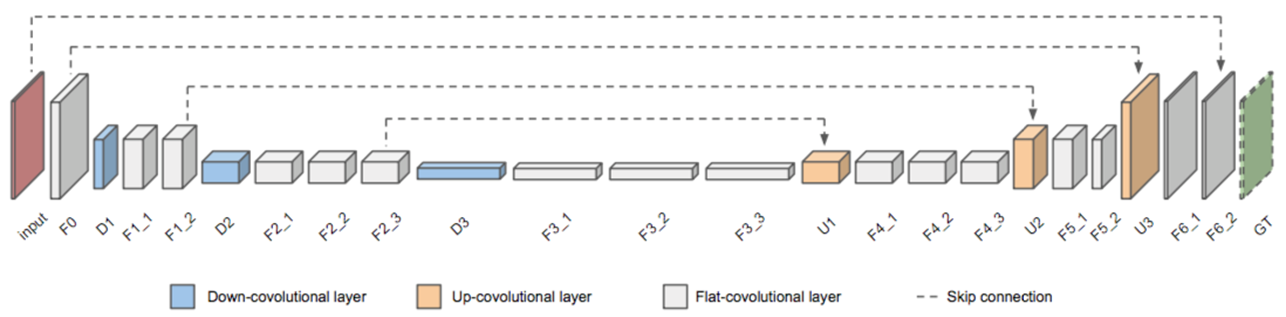
\includegraphics[width = 1\textwidth]{pic/deep_video_deblurring_cnn.png}
\caption{Structure of CNN used in Deep Video Deblurring\cite{su2016deep}}
\label{fig:deep_video_deblurring_cnn}
\end{figure}

Until now, the neural network is still a black box to researchers. No one could give a theoretical explanation, so I am not going to talk the details here.

\section{Overview of Existing Work}
In this section, I categorize the representative deblurring algorithms into $3$ kinds: 1) image priors; 2) kernel priors; 3) neural networks priors.
\subsection{Image Priors}
As mentioned above, I formulate the image deblurring objective function as following minimization problem:
\begin{equation}
\min_{\mathbf{l}, \mathbf{k}} \| \mathbf{b} - \mathbf{l} \otimes \mathbf{k} \| + \lambda\phi(\mathbf{l}) + \mu \rho(\mathbf{k}).
\label{eqn:objective_funtion}
\end{equation}

\textbf{\emph{Hyper-laplacian Prior}}\cite{krishnan2009fast}: this paper proposed a excellent non-blind image deblurring algorithm. Kernel is already given in non-blind deblurring so I only need to solve the first problem in Eqn.~\ref{eqn:blind_with_prior_alternative}. A hyper-laplacian image prior $\phi(\mathbf{l}) = \|\nabla \mathbf{l}\|_{\alpha}$ is proposed in this paper. As shown in Fig.~\ref{fig:hyper_laplacian}, the dark blue curve denotes the empirical image gradient distribution of natural images. The reason why hyper-laplacian is proposed is that the curve shape of  hyper-laplacian (green) is closet to the empirical one (dark blue). 
\begin{figure}[h!]
\centering
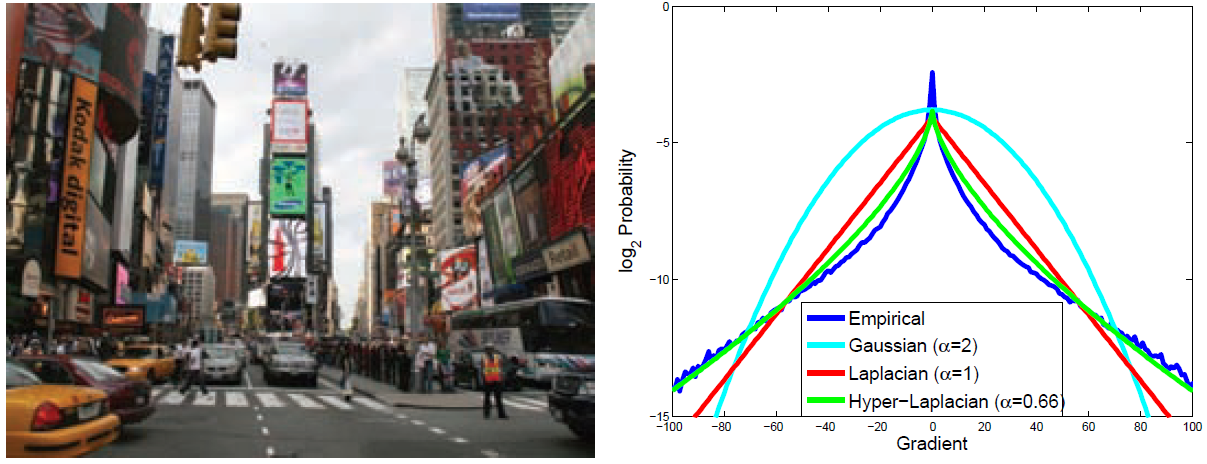
\includegraphics[width = 1\textwidth]{pic/hyper_laplacian.png}
\caption{Hyper-Laplacian Image Prior\cite{su2016deep}}
\label{fig:hyper_laplacian}
\end{figure}

However, solving the problem is still not trivial because the image prior $\phi(\mathbf{l}) = \|\nabla \mathbf{l}\|_{\alpha}$ is non-convex. The most commonly used method in image deblurring is to re-formulate the objective function again:
\begin{equation}
\min_{\mathbf{l}} \| \mathbf{b} - \mathbf{l} \otimes \mathbf{k} \|_2^2 + \lambda_1 \|\nabla \mathbf{l} - \mathbf{g}\|_2^2 + \lambda_2\|\mathbf{g}\|_{\alpha}.
\label{eqn:hyper_laplacian}
\end{equation}
Eqn.~\ref{eqn:hyper_laplacian} can be divided into two sub-optimization problems and solve alternatively:
\begin{equation}
\begin{cases}
\min_{\mathbf{l}} &\| \mathbf{b} - \mathbf{l} \otimes \mathbf{k} \|_2^2 + \lambda_1 \|\nabla \mathbf{l} - \mathbf{g}\|_2^2 \\
\min_{\mathbf{g}} &\lambda_1\|\nabla \mathbf{l} - \mathbf{g}\|_2^2 + \lambda_2\|\mathbf{g}\|_{\alpha}.
\end{cases}
\label{eqn:hyper_laplacian}
\end{equation}
The first minimization problem if Eqn.~\ref{eqn:hyper_laplacian} is a least-square problem which has closed-form solution. The second problem is difficult, so this paper used a lookup table solution. Besides, for some specific $\alpha = 0.5, 0.66$, exact analytical solutions can be found.

\textbf{\emph{Unnatural $L_0$ Sparsity Prior}}\cite{xu2013unnatural}: this paper proposed a blind image blurring algorithm with objective function as follows:
\begin{equation}
\min_{\mathbf{l}, \mathbf{k}} \| \mathbf{b} - \mathbf{l} \otimes \mathbf{k} \|_2^2 + \lambda \|\nabla \mathbf{l} \|_0 + \mu \| \mathbf{k} \|_2^2.
\label{eqn:l0_sparse}
\end{equation}
Similar as the last paper, this large optimization problem can be re-formulated into 3 small optimizations and solved alternatively:
\begin{equation}
\begin{cases}
\min_{\mathbf{l}} &\| \mathbf{b} - \mathbf{l} \otimes \mathbf{k} \|_2^2 + \lambda_1 \|\nabla \mathbf{l} - \mathbf{g}\|_2^2 \\
\min_{\mathbf{g}} &\lambda_1\|\nabla \mathbf{l} - \mathbf{g}\|_2^2 + \lambda_2\|\mathbf{g}\|_{0} \\
\min_{\mathbf{k}} &\| \nabla\mathbf{b} - \nabla\mathbf{l} \otimes \mathbf{k} \|_2^2 + \mu \|k\|_2^2
\end{cases}
\label{eqn:l0_sparse_alter}
\end{equation}


\subsection{Kernel Priors}

\subsection{Neural Networks Priors}

\section{Conclusion}
The conclusion goes here.



% by themselves when using endfloat and the captionsoff option.
\ifCLASSOPTIONcaptionsoff
  \newpage
\fi


% http://www.michaelshell.org/tex/ieeetran/bibtex/
\bibliographystyle{IEEEtran}
% argument is your BibTeX string definitions and bibliography database(s)
\bibliography{reference}


% that's all folks
\end{document}


